\documentclass[border=4pt,12pt]{standalone}
% House style for redrawn exam diagrams (diagram-v4: 0.4pt lines, filled -latex arrows, fine dashes; stipple and hatching drawn as real dots/lines (no PDF/SVG patterns, so they render in every browser and at any scale); transparent background). Every figure \input's this.
\usepackage{amsmath,amssymb}
\usepackage{txfonts}
\usepackage{pdfrender,xcolor}
% \halo{text}: label on shading. The shading stops just around each letter's outline (a thin knock-out that follows the
% glyphs, like the papers' typesetting), never a box. Owner: "I don't want a box around the text".
\newcommand{\halo}[1]{\leavevmode\rlap{\pdfrender{TextRenderingMode=2,LineWidth=2.2pt,LineJoinStyle=1,StrokeColor=white,FillColor=white}#1}#1}
\usepackage{tikz,pgfplots}
\pgfplotsset{compat=1.18}
\usetikzlibrary{arrows.meta,calc,angles,quotes,patterns,patterns.meta,intersections,positioning,decorations.markings,shapes.geometric}
% Stipple and hatching are drawn as actual dots / lines clipped to the region (path picture), NOT as pattern fills:
% SVG <pattern> fills vanish or blur when browsers scale the image, so the owner could not see the shading.
% Each dot is a 0.72pt square (keeps SVGs small; reads as a dot at print size). Dots sit on one global staggered grid, so neighbouring regions line up.
\makeatletter
\newdimen\ex@x \newdimen\ex@y \newdimen\ex@xa \newdimen\ex@ya \newdimen\ex@xb \newdimen\ex@yb \newcount\ex@row
\def\exam@stipplecolor{black!75}\def\exam@dotr{0.42pt}\def\exam@dotgap{2.5}
\def\ex@rowdots{\ifdim\ex@x<\ex@xb \pgfpathrectangle{\pgfqpoint{\dimexpr\ex@x-0.36pt\relax}{\dimexpr\ex@y-0.36pt\relax}}{\pgfqpoint{0.72pt}{0.72pt}}\advance\ex@x by \exam@dotgap pt\relax\expandafter\ex@rowdots\fi}
\def\exam@stipple{%
  \pgftransformreset% dots are sized in real points even inside scaled pictures
  \pgfpointanchor{path picture bounding box}{south west}\ex@xa=\pgf@x \ex@ya=\pgf@y
  \pgfpointanchor{path picture bounding box}{north east}\ex@xb=\pgf@x \ex@yb=\pgf@y
  \pgfsetfillcolor{\exam@stipplecolor}\pgfmathsetmacro\ex@h{\exam@dotgap/2}%
  \pgfmathtruncatemacro\ex@r{floor(\ex@ya/\ex@h)-1}\ex@row=\ex@r\relax
  \ex@y=\ex@r\dimexpr\ex@h pt\relax
  \loop\ifdim\ex@y<\ex@yb
    \pgfmathtruncatemacro\ex@c{floor(\ex@xa/\exam@dotgap)-1}\ex@x=\ex@c\dimexpr\exam@dotgap pt\relax
    \ifodd\ex@row \advance\ex@x by \ex@h pt\fi
    \ex@rowdots
    \advance\ex@y by \ex@h pt \advance\ex@row by 1
    \ifnum\numexpr\ex@row-(\ex@row/4)*4\relax=0 \pgfusepath{fill}\fi% flush every 4 rows: bounded TeX memory, few clip copies in the SVG
  \repeat\pgfusepath{fill}}
\newdimen\ex@d
\def\exam@hatch#1{% #1 = 1 for /, -1 for \ ; lines 45 degrees, 3pt apart
  \pgftransformreset
  \pgfpointanchor{path picture bounding box}{south west}\ex@xa=\pgf@x \ex@ya=\pgf@y
  \pgfpointanchor{path picture bounding box}{north east}\ex@xb=\pgf@x \ex@yb=\pgf@y
  \ex@d=\dimexpr\ex@yb-\ex@ya\relax \ex@x=\dimexpr\ex@xa-\ex@d\relax
  \loop\ifdim\ex@x<\ex@xb
    \ifnum#1>0 \pgfpathmoveto{\pgfqpoint{\ex@x}{\ex@ya}}\pgfpathlineto{\pgfqpoint{\dimexpr\ex@x+\ex@d\relax}{\ex@yb}}%
    \else \pgfpathmoveto{\pgfqpoint{\ex@x}{\ex@yb}}\pgfpathlineto{\pgfqpoint{\dimexpr\ex@x+\ex@d\relax}{\ex@ya}}\fi
    \advance\ex@x by 4.24pt
  \repeat
  \pgfsetlinewidth{0.4pt}\pgfsetstrokecolor{black}\pgfusepath{stroke}}
\def\examstipple{\exam@stipple}\def\examhatch{\exam@hatch}\def\examsetstipplecolor#1{\def\exam@stipplecolor{#1}}\def\examsetdotgap#1{\def\exam@dotgap{#1}}
\makeatother
% (legacy pattern kept for old files)
% staggered stipple like the NESA papers' dotted shading
\pgfdeclarepatternformonly{exam stipple}{\pgfpointorigin}{\pgfqpoint{2.2pt}{2.2pt}}{\pgfqpoint{2.2pt}{2.2pt}}{%
  \pgfpathcircle{\pgfqpoint{0.55pt}{0.55pt}}{0.42pt}\pgfpathcircle{\pgfqpoint{1.65pt}{1.65pt}}{0.42pt}\pgfusepath{fill}}
\tikzset{
  every picture/.style={line width=0.6pt, >={Latex[length=2mm,width=1.3mm]}},
  curve/.style={line width=0.6pt},
  open arrow/.style={-{Latex[length=2mm,width=1.3mm]}},  % owner: filled -latex heads everywhere, no open chevrons
  aux/.style={dash pattern=on 2pt off 1.5pt, line width=0.6pt},
  shade/.code={\def\exA{#1}\def\exB{none}\ifx\exA\exB\else\pgfkeysalso{fill=black!18}\fi},
  shade/.default=on,
  shade dots/.style={fill=none, path picture={\examstipple}},
  stipple color/.code={\examsetstipplecolor{#1}},
  stipple gap/.code={\examsetdotgap{#1}},
  shade dense dots/.style={fill=none, stipple gap=1.6, path picture={\examstipple}},
  shade hatch/.style={fill=none, path picture={\examhatch{1}}},
  shade hatch reverse/.style={fill=none, path picture={\examhatch{-1}}},
  shade solid/.style={fill=black},
  pt/.style={circle, fill, inner sep=1.1pt},
  open pt/.style={circle, draw, fill=white, inner sep=1.1pt},
}
\pgfplotsset{
  exam axes/.style={axis lines=middle, axis line style={->}, xlabel={$x$}, ylabel={$y$},
    xlabel style={anchor=west}, ylabel style={anchor=south}, tick label style={font=\small},
    every axis plot/.append style={line width=0.6pt, black}, samples=200, clip=false,
    enlargelimits=false, axis on top},
}

\begin{document}
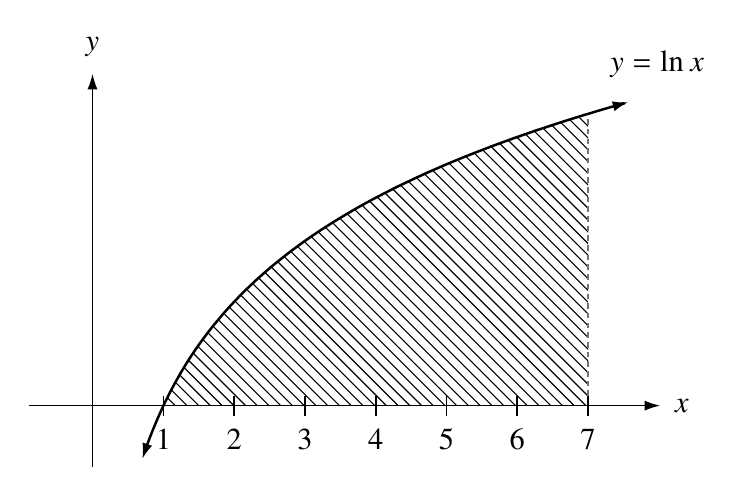
\begin{tikzpicture}[x=0.0127cm,y=-0.0127cm, every node/.style={font=\fontsize{11}{13}\selectfont}]
\fill[shade hatch reverse] plot[smooth] coordinates {(163.0,384.0) (173.9,362.5) (184.8,343.8) (195.7,327.1) (206.6,312.1) (217.5,298.4) (228.4,285.9) (239.2,274.4) (250.1,263.6) (261.0,253.6) (271.9,244.3) (282.8,235.4) (293.7,227.1) (304.6,219.2) (315.5,211.7) (326.4,204.6) (337.3,197.7) (348.2,191.2) (359.1,185.0) (370.0,179.0) (380.8,173.2) (391.7,167.6) (402.6,162.3) (413.5,157.1) (424.4,152.1) (435.3,147.3) (446.2,142.6) (457.1,138.0) (468.0,133.6) (478.9,129.3) (489.8,125.2) (500.7,121.1) (511.6,117.2) (522.4,113.3) (533.3,109.6) (544.2,105.9) (555.1,102.3) (566.0,98.9) (576.9,95.4) (587.8,92.1)} -- (587.8,384) -- cycle;
\draw[aux,black!55] (587.8,384) -- (587.8,92.1);
\draw[->] (28,384) -- (660,384);
\draw[->] (92,445) -- (92,52);
\draw (163.0,374) -- (163.0,394);
\draw (233.8,374) -- (233.8,394);
\draw (304.6,374) -- (304.6,394);
\draw (375.4,374) -- (375.4,394);
\draw (446.2,374) -- (446.2,394);
\draw (517.0,374) -- (517.0,394);
\draw (587.8,374) -- (587.8,394);
\node at (163.0,418) {$1$};
\node at (233.8,418) {$2$};
\node at (304.6,418) {$3$};
\node at (375.4,418) {$4$};
\node at (446.2,418) {$5$};
\node at (517.0,418) {$6$};
\node at (587.8,418) {$7$};
\draw[<->, line width=0.9pt] plot[smooth] coordinates {(141.8,437.5) (147.2,421.8) (152.7,407.6) (158.2,394.6) (163.6,382.7) (169.1,371.6) (174.6,361.3) (180.0,351.7) (185.5,342.6) (190.9,334.1) (196.4,326.0) (201.9,318.3) (207.3,311.1) (212.8,304.1) (218.3,297.5) (223.7,291.1) (229.2,285.0) (234.7,279.1) (240.1,273.5) (245.6,268.0) (251.1,262.8) (256.5,257.7) (262.0,252.8) (267.5,248.0) (272.9,243.4) (278.4,239.0) (283.9,234.6) (289.3,230.4) (294.8,226.3) (300.2,222.3) (305.7,218.4) (311.2,214.6) (316.6,210.9) (322.1,207.3) (327.6,203.8) (333.0,200.4) (338.5,197.0) (344.0,193.7) (349.4,190.5) (354.9,187.3) (360.4,184.2) (365.8,181.2) (371.3,178.2) (376.8,175.3) (382.2,172.5) (387.7,169.7) (393.2,166.9) (398.6,164.2) (404.1,161.6) (409.6,159.0) (415.0,156.4) (420.5,153.9) (425.9,151.4) (431.4,149.0) (436.9,146.6) (442.3,144.2) (447.8,141.9) (453.3,139.6) (458.7,137.4) (464.2,135.1) (469.7,133.0) (475.1,130.8) (480.6,128.7) (486.1,126.6) (491.5,124.5) (497.0,122.5) (502.5,120.5) (507.9,118.5) (513.4,116.5) (518.9,114.6) (524.3,112.7) (529.8,110.8) (535.2,108.9) (540.7,107.1) (546.2,105.3) (551.6,103.5) (557.1,101.7) (562.6,99.9) (568.0,98.2) (573.5,96.5) (579.0,94.8) (584.4,93.1) (589.9,91.5) (595.4,89.8) (600.8,88.2) (606.3,86.6) (611.8,85.0) (617.2,83.5) (622.7,81.9) (628.2,80.4)};
\node at (657,42) {$y=\ln x$};
\node at (92,25) {$y$};
\node at (681,384) {$x$};
\end{tikzpicture}
\end{document}